% set home directory
\providecommand{\homedir}{..} 
% load the preamble of main.tex by subfiles
\documentclass[\homedir/main.tex]{subfiles}
% ##############################################################################
\begin{document}
% set chapter numbering to work correctly even when separate compilation using subfile
\setcounter{chapter}{2}
% ##############################################################################
\chapter{理論}\label{chap:theories}
ニューラルネットワークを用いたStyle Transferの研究では,
畳み込みニューラルネットワークやGenerative Adversarial Network を
応用したモデルや手法がよく用いられている.
そこで,本研究の前提知識として
\cref{sec:cnn}では畳み込みニューラルネットワークについて説明し,
\cref{sec:gan_and_its_improvements}ではGenerative Adversarial Networkと
その改良について説明する.

また本章の最後の\cref{sec:projective_transformation}では,
ある文字列の形状の歪みを別の文字列へと転写するために本研究で用いた射影変換について説明する.

% ##############################################################################
\section{畳み込みニューラルネットワーク}\label{sec:cnn}
畳み込みニューラルネットワーク(Convolutional Neural Network: CNN)とは,
畳み込み(Convolution)演算をはじめとする画像処理の技法を
ニューラルネットワークに応用したものである.
そのため,CNNは他のニューラルネットワークに比べて
画像データを扱うことに長けており,主に画像認識の分野で広く用いられている.

先述したように,CNNには画像処理の技法が応用されているため,
CNNを十分に理解するためには画像処理の技法の知識が必要不可欠だと考える.
ゆえに,コンピュータ上での画像データの扱いと,
画像処理の技法について先に説明する.

% =====
初めに,コンピュータ上での画像データの扱いについて説明する.

一般に,コンピュータ上における画像データのフォーマットは
「ラスタ形式」のものと「ベクタ形式」のものの二つに大別される.
これらのうち,ラスタ形式では画像を構成する各ピクセルの色に対応する数値を
全て格納した配列\footnote{但し,圧縮については考慮しないとする.}として画像データを表現する.
なお,この「ピクセルの色に対応する数値」は「画素値」や「ピクセル値」などと呼ばれている.
一方,ベクタ形式では画像に描かれているものを表現するための
座標や数式などのあつまりとして画像データを表現する.
よって,写真のように色や形状が複雑な画像の場合,
ベクタ形式よりもラスタ形式が適していると言える.
また,ラスタ形式の画像データはピクセル値の配列であるため,
コンピュータ上で画像データのピクセル値を参照した処理を行う際にも,
ベクタ形式よりもラスタ形式が適していると言える.

以下では,絵や写真を含む様々な画像のコンピュータを用いた処理について考えるため,
単に画像と言った場合はラスタ形式の画像を指すものとする.

ここで,後の説明のために画像の「チャネル(channel)」について説明する.

その前提として,白黒でない画像のピクセル値が複数の成分をもつことを確認する.
白黒画像では,輝度を表すスカラをピクセル値とすれば良く,ピクセル値の成分は一つでよい.
しかし,カラー画像では色の指定に三原色\footnote{光の三原色である赤(R)・緑(G)・青(B)}の
混合比率が必要なので,ピクセル値には三つの成分が必要になる.
さらに,透過画像では三原色に対応した三つの成分に加え,
ピクセルの不透明度\footnote{アルファ値とも呼ばれる}が必要なので,
ピクセル値には計四つの成分が必要になる.
以上から,白黒でない画像のピクセル値が複数の成分をもつことが確認できた.

このことから,白黒でない画像は複数の白黒画像で構成されているものだとみなせるが,
このように「ある画像中の特定の成分を抽出してできる白黒画像」はチャネルと呼ばれる.
例えば,通常のカラー画像は赤のチャネル,緑のチャネル,青のチャネルの
三つの白黒画像から構成されているとみなせる.

なお,CNNによって処理されている途中の画像は,
通常の画像より遥かにチャネル数が多い.
これは各チャネルが元画像の何らかの特徴を表すためである.
(詳しくは後述する.)

% =====
次に,画像処理の技法のうち畳み込み演算を用いたフィルタリングについて説明する.

畳み込み演算を用いたフィルタリングとは,
対象の画像と「カーネル\footnote{画像フィルタなどとも呼ばれる}」
と呼ばれる画像との畳み込み演算である.
そのため,フィルタリングに用いるカーネルがどのようなものかによって
フィルタリング後の結果が大きく左右される.(詳しくは後述する.)

ここからは,\cref{fig:img_to_be_filtered}に示す\(5 \times 5\)ピクセルの白黒画像を対象に,
\cref{fig:conv_ker}に示すカーネルを用いてフィルタリングする場合を例にして動作を説明する.

\begin{figure}[h]
    \centering
    \begin{minipage}[b]{0.375\linewidth}
        \centering
        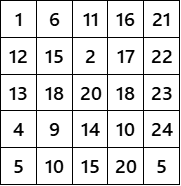
\includegraphics[keepaspectratio, scale=0.7]{image_to_be_filtered.png}
        \subcaption{フィルタリング対象の画像}
        \label{fig:img_to_be_filtered}
    \end{minipage}
    \begin{minipage}[b]{0.375\linewidth}
        \centering
        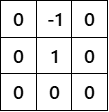
\includegraphics[keepaspectratio, scale=0.7]{conv_kernel.png}
        \subcaption{フィルタリングに用いるカーネル}
        \label{fig:conv_ker}
    \end{minipage}
    \caption[フィルタリングの例に用いる画像とカーネル]{
        例として用いる画像とカーネル \linebreak
        (文献\cite{fujita2017}のp157図8.2をもとに作成)
    }
    \label{fig:conv_operand}
\end{figure}

\noindent
対象の画像とカーネルとの畳み込み演算では
次の\cref{fig:conv_calc_precess}に示すような処理が基本となる.

\begin{figure}[h]
    \centering
    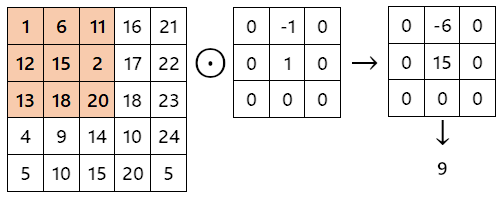
\includegraphics[keepaspectratio, width=0.8\linewidth]{conv_calc_precess.png}
    \caption[畳み込み演算の過程]{
        畳み込み演算の過程 \linebreak
        (文献\cite{fujita2017}の図p158図8.2をもとに作成)
    }
    \label{fig:conv_calc_precess}
\end{figure}

\newpage \noindent
\cref{fig:conv_calc_precess}に示した処理は次の2つのステップに分けられる.
\begin{enumerate}[label=\textbf{Step\arabic*.}]
    \setlength{\leftskip}{0.5cm}
    \item フィルタリング対象の画像からカーネルと同じサイズの小さな画像を切り出す.\\
          また,以下ではここで切り出した小さな画像のことを「パッチ」と呼ぶとする.\\
          なお,\cref{fig:conv_calc_precess}では切り出すパッチ内のピクセルに色を付けて示した.
    \item Step1で切り出したパッチとカーネルの標準内積をとる.\\
          なお,\cref{fig:conv_calc_precess}では標準内積を要素積と総和の二段階に分けて表記した.
\end{enumerate}

対象の画像とカーネルとの畳み込み演算とは,
パッチを切り出す範囲を一定幅で移動させつつ上記の処理を繰り返し実行し,
得た数値を順に並べて新たな画像を作成する処理である.
なお,この「パッチを切り出す範囲をずらす幅」は
ストライド\footnote{スライド幅とも呼ばれる}と呼ばれている.

例えば,次の\cref{fig:conv_result}は\cref{fig:conv_operand}の組を
ストライドを1として畳み込み演算した結果である.

\begin{figure}[h]
    \centering
    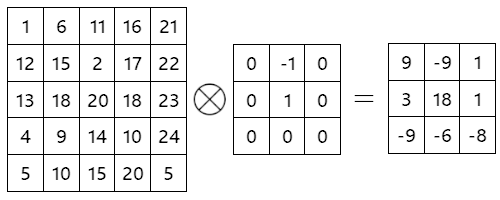
\includegraphics[keepaspectratio, width=0.8\linewidth]{conv_result.png}
    \caption[畳み込み演算の結果]{
        畳み込み演算の結果 \linebreak
        (文献\cite{fujita2017}の図p158図8.2をもとに作成)
    }
    \label{fig:conv_result}
\end{figure}

\cref{fig:conv_result}を見ると分かるように,
カーネルとの畳み込み演算を行うと画像のサイズは元画像より小さくなる.
そこで,出力画像サイズの担保のため,
畳み込み演算の実行前に元画像を拡張する手法が用いられることがある.
この手法は「パディング」と呼ばれている.

また,カーネルとの畳み込み演算の過程で標準内積が用いられていることから分かるが,
畳み込み演算を用いたフィルタリングはカーネルとの相関
\footnote{
    CNNなどの分野で畳み込み演算と呼ばれている演算は,厳密に言えば数学の分野では相互相関にあたる.\\
    本来の畳み込みは系列の積をとる際,逆順で積をとるように定義されている.
}
の計算を意味している.

% =====
続いて,画像処理の技法のうちプーリング(Pooling)について説明する.

プーリングとは,入力画像の特徴を最大限保存しつつ画像サイズを縮小する処理である.

ダウンサンプリングとも呼ばれる
TODO:プーリングの説明

% =====
最後に,以上の説明を踏まえてCNNについて説明する.

TODO:まとめとCNN

% ##############################################################################
\section{Generative Adversarial Networkとその改良}\label{sec:gan_and_its_improvements}
\subsection{Generative Adversarial Network}\label{sec:gan}
Generative Adversarial Network(GAN)とは,
「乱数などの入力を元に新たなデータを生成するネットワーク」であるGeneratorと
「入力されたデータがGeneratorが生成したデータか,
訓練データかを判断するネットワーク」であるDiscriminatorの
二つのネットワークからなる生成モデルである.
GANは\citeyear{NIPS2014_5ca3e9b1}年に
Goodfellowら\cite{NIPS2014_5ca3e9b1}によって提案されて以降,
幅広い分野で応用されてきたが,
本研究で扱うStyle Transferもそうした応用先の一つである.


TODO:



\subsection{Wasserstein GAN}\label{sec:wgan}
\cref{sec:gan}で説明したGANには次のような問題点があることが知られている.

TODO:

以上のようなGANの問題点を解決するため,
Wasserstein GAN(WGAN)は
Arjovskyら\cite{pmlr-v70-arjovsky17a}によって提案された.
GANの損失関数をWasserstein距離を用いたものに変更した

TODO:
WGANでは,

\subsection{WGAN with a gradient penalty}\label{sec:wgan_gp}
\cref{sec:wgan}で説明したWGANはGANの問題点を改善したものの完璧ではない

TODO:

Gulrajaniら\cite{NIPS2017_892c3b1c}は,
WGANにgradient penalty項を追加することを提案した.
これはgradient penaltyをgpと略してWGAN-gpと呼ばれている.

% ##############################################################################
\section{射影変換}\label{sec:projective_transformation}

TODO:

% ##############################################################################
\printBibForSubfiles
\end{document}